% Generated from work/deck/chart-data-en.mjs; numeric data preserved.
% Input in a column; rocpr is intended for full frame width.
\begingroup
\definecolor{blueplot}{HTML}{4E79A7}
\definecolor{redplot}{HTML}{D95F59}
\definecolor{inkplot}{HTML}{111111}
\definecolor{lightplot}{HTML}{8FB8DA}
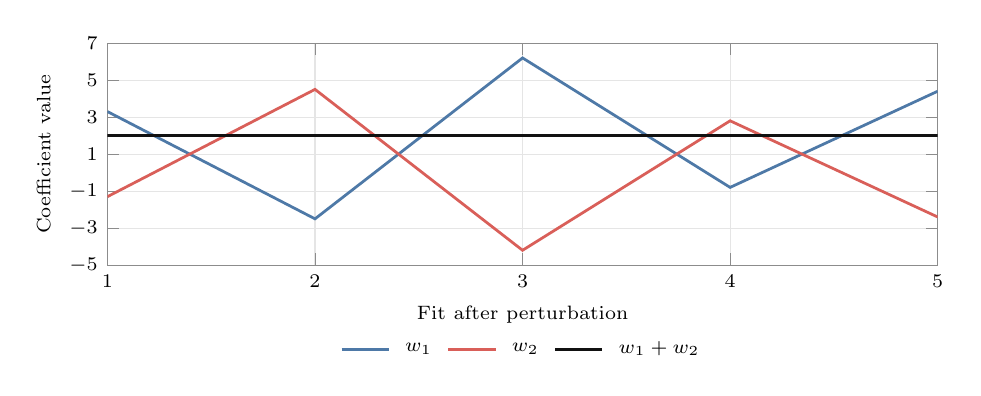
\begin{tikzpicture}
\begin{axis}[
width=\linewidth,
height=4.4cm,
font=\scriptsize,
tick label style={font=\scriptsize},
label style={font=\scriptsize},
axis line style={black!45},
tick style={black!45},
grid=major,
grid style={black!10},
xmin=1,
xmax=5,
ymin=-5,
ymax=7,
xlabel={Fit after perturbation},
ylabel={Coefficient value},
scaled ticks=false,
tick label style={/pgf/number format/fixed},
clip=true,
unbounded coords=jump,
legend style={font=\scriptsize,draw=none,fill=none,at={(0.5,-0.29)},anchor=north,legend cell align=left,column sep=0.12cm,row sep=0.03cm},
legend columns=-1,
xtick={1,2,3,4,5},
ytick={-5,-3,-1,1,3,5,7}
]
\addplot+[no marks,draw=blueplot,line width=1pt] coordinates {(1,3.3) (2,-2.49999999999) (3,6.19999999999) (4,-0.799999999993) (5,4.39999999999)};
\addlegendentry{$w_1$}
\addplot+[no marks,draw=redplot,line width=1pt] coordinates {(1,-1.3) (2,4.49999999999) (3,-4.19999999999) (4,2.79999999999) (5,-2.39999999999)};
\addlegendentry{$w_2$}
\addplot+[no marks,draw=inkplot,line width=1pt] coordinates {(1,2) (2,2) (3,2) (4,2) (5,2)};
\addlegendentry{$w_1+w_2$}
\end{axis}
\end{tikzpicture}
\endgroup
